% $Id: p008.tex,v 1.33 2011/11/29 16:45:35 rbj Exp $
% bibref{rbjp008} pdfname{p008} 

\documentclass[10pt,titlepage]{book}
\usepackage{makeidx}
\usepackage{graphicx}
\usepackage[unicode,pdftex]{hyperref}
\pagestyle{headings}
\usepackage[twoside,paperwidth=5.25in,paperheight=8in,hmargin={0.75in,0.5in},vmargin={0.5in,0.5in},includehead,includefoot]{geometry}
\hypersetup{pdfauthor={Roger Bishop Jones}}
\hypersetup{colorlinks=true, urlcolor=red, citecolor=blue, filecolor=blue, linkcolor=blue}
\usepackage{html}
\usepackage{paralist}
\usepackage{relsize}
\usepackage{verbatim}
\bodytext{BGCOLOR="#eeeeff"}
\makeindex
\newcommand{\indexentry}[2]{\item #1 #2}
\newcommand{\glossentry}[2]{\item #1 {\index #1 #2}}
\newcommand{\ignore}[1]{}
\def\Product{ProofPower}
\def\ouml{\"o}
\def\auml{\"a}

\title{A Conversation\\{\small between}\\Carnap and Grice\\{\small as it might have been}}
\author{Roger~Bishop~Jones\\\small{and}\\J.L.~Speranza}
\date{\ }

\begin{document}
\frontmatter
                               
\begin{titlepage}
\maketitle

\vfill

%\begin{abstract}
%A speculation about what the fundamental differences between the philosophies of Rudolf Carnap and Paul Grice might have been had they survived into the twenty first century.
%\end{abstract}

\begin{centering}

{\footnotesize
\begin{verbatim}

Library of Congress Cataloging-in-Publication Data

Jones, Roger Bishop
Speranza, J. L.
    A Conversation between Grice and Carnap /
          Roger Bishop Jones and J.L. Speranza
     p. cm.
ISBN 1-40......
  1. Carnap, Rudolf.
  2. Grice, H. P. (H. Paul)

\end{verbatim}

\copyright\ Roger~Bishop~Jones and J.L.~Speranza;
}%footnotesize

\end{centering}
\end{titlepage}

\setcounter{tocdepth}{2}
{\parskip-0pt\tableofcontents}
\listoffigures

\mainmatter

\addcontentsline{toc}{section}{Preface}

\section*{Preface}
This work was the result of our shared interest in twentieth-century  
philosophy. While centred around an exegesis of historical nature of our  
mentors, it aims at more than that. Indeed, we take Carnap and Grice as  paradigms 
of two types of doing philosophy, and it is our intention to present  our 
joint endeavour as proof that collaboration from historically different  
paradigms is indeed feasible and fruitful.
 
Roger Bishop Jones continues a line of analytic philosophy whose closest predecessor
is that of Rudolf Carnap, and thus has a vital interest in a sound assessment of the
merits of Carnap's philosophy, its defence against ill-founded criticisms, and in
future developments in similar spirit.
One way of progressing these interests is through this dialogue with Speranza,
in which we explore the relationship between the philosophies of Carnap and Grice.

J. L. Speranza has presented his views on the philosophy of H. P. Grice in  
various fora, and is happy to have been able to further his exegesis of his 
 mentor from a strict comparative perspective. The overlap with various  
points in Carnap's career, he believes, sheds light on the Gricean programme 
in  ways which a monographic study would not. 
 
A comparison of philosophers is built on the need of a common ground: a  
lingua franca. While both Carnap and Grice shared the 'analytic' idiom, the  
details of each of their idiolects is worth examining. And it is in this 
common  idiom that progress, as regards the second goal of our endeavour, will  
be, we trust, expressed.  

\chapter{Introduction}

{\it [This chapter as a whole still needs a lot of work before it gets close to saying what I have in mind. (RBJ)]}

In considering how a conversation between Carnap and Grice might go, the possibility arises that it might not go at all.
Sometimes dialogue between philosophers does break down, and there is evidence of such breakdowns by which Carnap and Grice might easily have been affected.

Sometimes the alienation appears as a clash of cultures.
At its starkest such a clash is shown in the polemics of Bertrand Russell, an important (possibly the most important) influence shaping the philosophy of Carnap, who said in relation to ordinary language philosophy (of which Grice was a defender), speaking of ``the cult of common usage'' delivered a scathing and rather unphilosophical indictment of what he understood by that phrase, and of the reasons why a philosopher might adopt it.

That Carnap stood by Russell's side in this (except perhaps in the vitriolic and \emph{ad hominem} character of the attack) may be seen by reading his intellectual autobiography \cite{carnap63a}, in which he describes himself as having been inspired by Russell to devote his life to the application of the new logical methods to the analysis of science.
Carnap is explicit in regarding philosophy as confined to establishing purely logical results, and as considering the features of ordinary languages as falling outside this domain.

By contrast, Grice comes from one of (if not {\it the}) most important centres of the kind of philosophy which Russell abjured.
Just as Carnap saw himself as engaged in a collaborative venture furthering Russell's conception of scientific philosophy, Grice was also, in perhaps less doctrinaire a way, a team player who rose to the defence of ``ordinary language philosophy'' and of metaphysics.

Working for us in our hope of constructive engagement is the character of the two men.
Both men preferred a collaborative striving to move forward in the search for understanding, both of how things are and how they might be, but also of methods which facilitate progress.
Neither man was wholly consistent with the expectations which we might harbour on the basis of this coarse characterisation of their intellectual roots.

Carnap, though an early and vigorous advocate of the elimination of metaphysics, developed a narrow conception of metaphysics which ultimately proscribed no coherent language for which a pragmatic rationale could be mounted.
His early narrow delineation of philosophy as involved exclusively in the promulgation of logical propositions (alongside various linguistic and methodological {\it proposals}), eventually faded away, leaving no desire to prescribe limits to philosophy.
The pragmatic admission of much that one might suppose to be metaphysics was accompanied by more conciliatory language in relation to other important domains, such as that of ethics.
These were no longer said to be meaningless, but rather as lacking ``cognitive content'', the significance of which might be thought more moderate.
Insofar as Carnap can properly be called a ``positivist'' (which he later doubted himself) it was a particularly innocuous kind of positivism, with the dogmatic teeth drawn.
The ``minimalisms'' which later concerned Grice, many of which are heavily associated with positivistic dogma, became in the later Carnap (of which there are clear precursors from his earliest years) options in a liberal pluralistic framework, rather than closed dogmas.

Grice too can be seen, at the same time as defending ``ordinary language'' philosophy and metaphysics against their detractors, failed to embody Russell's caricature of Aristotelian scholars unwilling to embrace modern logic.

Notwithstanding that neither philosopher complied with the radical attributions which might have made them irreconcilable, we may still fear differences sufficient for a conversation to be difficult and productive.
We will examine in detail both the areas where common ground might prove hardest to find, and those where the opportunity for constructive collaboration might be best, but speculate in advance that our greatest difficulty may lie in the desire of Carnap to see radical change in the way in which philosophy is undertaken, in which formal logic would play a prominent role, when set against a preoccupation on the part of Grice, simply to understand certain related matters, most conspicuously {\it meaning}, without desiring, and possibly while resisting, any leanings for reform.


\section{Conflict and Collaboration}

We are looking to learn by considering how in a contemporary context, allowing possibly for some further development which might have taken place since we last heard from them, a conversation between Carnap and Grice might be secured.
Our interest is not in the kind of clash which might occur if things went much worse than we might hope, and each philosopher was obdurate in seeing and rejecting what he found worst in his adversary.

The distinction between the kind of conversation which concerns us and the kind of conflict which does not is of interest in itself, for it connects with elements in the work of each philosopher, and possibly with ideals for how philosophy might be.

One way to draw the distinction is as a distinction between philosophy as a ``gladiatorial'' conflict and as a conversational collaboration.
\footnote{
Our gladiatorial-conversational dichotomy bears some resemblance with  
Grice's own epagogic-diagogic one. As Grice became wiser (by 1986, or so) in  
``Life and Opinions'' he would reminisce on how he grew out of a mere  
'gladiatorial' or 'epagogic' as he prefers view of philosophy as imbued with  
counterexamples.
He was the master of the counterexample, and this struck back  
with a vengeance -- as per McKay\cite{mackay72} who calls Grice totally ad-hoc.
An ad-hoc theory, for McKay is one built ONLY to cope with counterexamples.
As Harrison notes \cite{harrison79} Grice on meaning rivals rule-utilitarianism in being 'the thesis most beguiled with 
counterexamples'.
So he knew what he was talking about.
In later days, as we say, he turned  'diagogic'.
He would like to see a thesis as propounded 'by its own merits' rather than as a 'gladiatorial' defeat of its opponents.
Diagoge is the Greek  term which connects with our more conversational use of 'conversational'.}

Here are some features:

\begin{description}

\item[gladiatorial] \ 

In gladiatorial philosophy, one engages with one or more opponents and aims to prevail.
An outright defeat conceded by the opponent is best, but a kind of point victory is better than nothing.
It is not the purpose of the exercise to understand your opponent or to learn anything from him (you already know better than he does).
It is not necessary to criticise the position he actually holds, this would often involve considerable effort in first coming to an understanding of that position.
It is necessary only to refute what he says, understood in whatever way is most convenient for a convincing dismissal.

\item[conversational] \ 
Conversation philosophy is a game played by two or more philosophers having a common interest in some subject matter who believe that through dialogue they can come to understand that subject better than they otherwise might.
The idea is that seeing this problem from another persons point of view will enrich ones own understanding, even if that point of view is not necessarily ``better'' than your own.
To obtain this benefit it may be necessary to invest considerable effort in coming to an understanding of the others position, and in conveying to him an understanding of your own.
Not all of it, the bits which bear upon the issues.

Unless all partners are committed to this process it will not work.
\end{description}

\ignore{

It is my perception, that in philosophical discussion on the Internet, it is very difficult to achieve what I have called a conversational dialogue.
It is the norm rather than the exception that people from the first assume that they understand what you are saying, and one may then find many occasions to complain that an adversary criticises a position that one has never held.

This is however, not a problem exclusive to the Internet fringe.
It is pervasive in the writings of professional philosophers that a philosopher will criticise an opponent by attacking a position which he has never held.
If the philosopher is at the van of a new philosophical trend this can be done with impunity, readers sympathetic to the new philosophical trend will not trouble to check the accuracy of the picture presented of some obsolescent point of view.

Sometimes a failure to converse is not due to bad faith.
Two philosophers earnestly wishing to understand each other may nevertheless fail for reasons which are mysterious and may possibly be insurmountable, and we shall touch upon some of these.

The point of this little diatribe is to explain that one of our aims in discussing Carnap and Grice here is to explore whether they might have had a conversation, and whether some of the ideas of metaphysical positivism might help in providing a basis for that dialogue.
To say some things on either side which might help to make conversation possible.
Locating the points at which incomprehension, may possibly facilitate their isolation, and permit conversation elsewhere.

}%ignore


\section{Dogma and Scepticism}

There is more to our discussion here, of the nature of genuine conversation and how it may fail, than may appear at first glance.

It is not just about the kind of conversation we are considering here between Carnap and Grice, one in which we seek common ground on which they both might have built.

The pathologies of `gladiatorial' philosophical conflict may be seen as arising from or exhibited in various kinds of dogmatism.
The gladiatorial stance may often have been provoked by to great and too uncompromising a conviction on the part of the gladiator in the truth of the theories which he defends by attacking their opponents.
The gladiator need only understand his opponent only as well as is needed to launch an attack which will convince others even if it does so in part by misrepresentation, or as a result of misunderstanding.
Since he does not seek learn from his opponent, he need only understand him well enough to mount an attack.

An attack which depends upon a misunderstanding or misrepresentation may be just as difficult to parry than one soundly based, and probably be easier to construct (especially if the position attacked is essentially sound).
One way of carrying through such an attack is simply to disregard what you know your opponent to mean, by concentrating on ``the'' meaning of what he says.
This is a kind of terminological dogmatism.

\section{Reconciling Carnap and Grice}

Carnap and Grice are the representatives of two substantially divergent trends in analytic philosophy but each may be seen as a moderating influence.
The dialogue between these traditions leans away from the conversational toward the gladiatorial.
To secure our conversation we have to be prepared to pass over some of the view of each philosopher.
The connection suggested between conflict and certain kinds of dogmatism may help us to identify aspects of the philosophies of Carnap and Grice whose moderation would facilitate constructive conversation.
Negative dogmas and terminological dogmas are the greatest source of danger, because they may easily be mistaken for a reasonable scepticism, or a sound analysis of language as it is.

In order to reconcile the philosophies of Carnap and Grice so that they might move on together toward \emph(The City of Eternal Truth), we propose first to consider the philosophy of each from the perspective of the other, to locate the points at which from that point of view may appear dogmatic, and to consider whether these apparent sticking points are essential to the important insights which the philosopher uncovers.
Alongside this, it is important to locate terminological divergence.
It is important to distinguish between substantive disagreements, and differences in usage, even if there might be a substantial question about the merits of the alternative terminologies.

\section{The City of Eternal Truth}

This is an ideal toward which we represent both Carnap and Grice as working.
That there is such a common ideal is moot, the interest in the present work being in presenting a conception of such an ideal on which they might conceivably have converged, after a very long conversation.

\begin{figure}
\centering
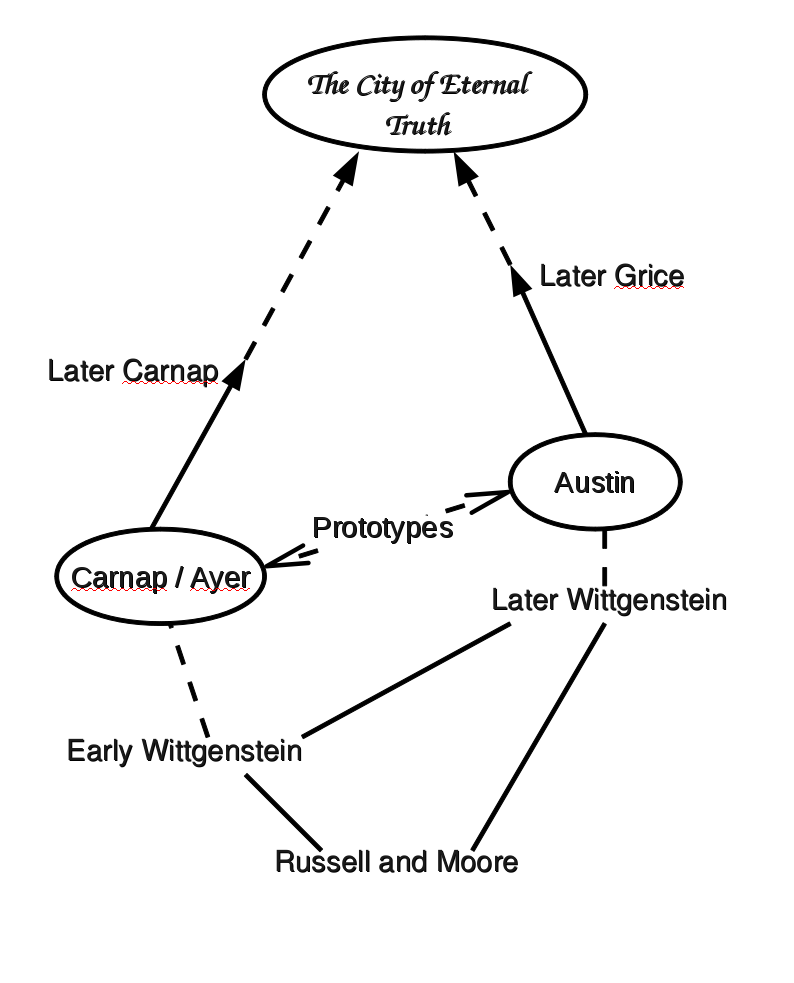
\includegraphics[height=3in]{p008a.png}
\caption{An Approach to The City of Eternal Truth \label{ApproachToCity}}
\end{figure}



We envisage them as approaching this common goal from opposite ends of a spectrum of analytic philosophy in the twentieth century both extremes of which are related to if not actually occupied by the two philosophies of Ludwig Wittgenstein.
These two extremes succeed in differing so widely primarily through the offices of certain dogmas.
Carnap and Grice begin at or near these extremes in their early philosophies, but moderate the dogmas as their philosophies mature.
It is this process of moderation, consisting primarily in the replacement of crude dogmas with more subtle and flexible insights, which we perceive, were it to be continued, might ultimately lead both to that same ``City of Eternal Truth''.

We do not intend to suggest by this picture (figure \ref{ApproachToCity}) that the philosophies of Carnap and Grice are purely or even predominantly derived from those of Wittgenstein.
The picture should be taken with some salt.

For our purposes no detailed discussion of Wittgenstein will be necessary, and it may be as well to think instead in terms of the even more simplistic figure \ref{Simpler Approach}.

\begin{figure}
\centering
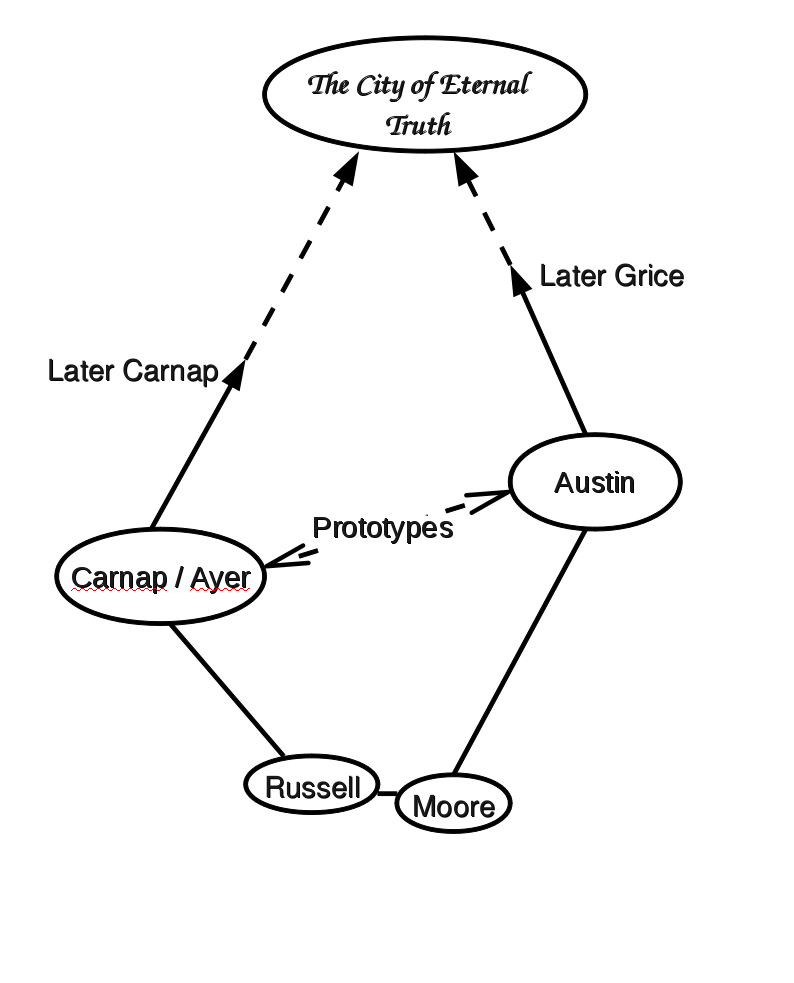
\includegraphics[height=3in]{p008b.png}
\caption{A Simpler Picture \label{Simpler Approach}}
\end{figure}

\subsection{Longitudinal Perspective}

Note the chronological development.
It all started in Cambridge with G. E. Moore and B. A. Russell.
\footnote{A good source for this is Ayer's book, \emph{Moore and Russell: the analytical
heritage} \cite{ayer1971}.}

This is then followed by whom Russell referred to as ``the Austrian
engineer'': Ludwig ``Witters'' as J. L. Austin would call him (``Some like
Witters, but Moore's still MY man'').
There are at least TWO Witters: the early and the later (never late).

The connection is between the early Wittgenstein (of the Tractatus, that is) and both Carnap and Ayer.
Ayer having sent to Vienna by his once tutor in Oxford: Gilbert Ryle.

At the \emph{same} time, there's the influence of the later Wittgenstein on Austin and Grice.

Grice does quote directly from ``Philosophical Investigations'' in WoW:i\cite{grice89}.
The Prolegomena that he waited so long to publish (because it IS a provocative piece).
It was via an Oxonian connection.
G. E. M. Anscombe, after all, had translated the Philosophical Investigations and published them back in Oxford
where she was teaching.

Then we have indeed the later Carnap, and the still later Grice.
Carnap died in Sept. 1970 -- in Santa Monica. -- Grice will survive him for
some 18 years, but then he was younger.

``The city of eternal truth'' is the name Grice uses for the destination of his pilgrimage.

\subsection{Latitudinal Perspective}

The latitudes may be thought of a little like the very imperfect left/right characterisations of political parties, but in this case of philosophical systems or postures.

On the left we have radical positivism (often said to be an \emph{anti-philosophical} philosophy) and the Tractatus (close enough to be blamed, perhaps unfairly, for logical positivism), on the right Wittgenstein's radical rejection of his Tractatus characterised not only by a broader conception of language and a complete rejection of much of what is found on the left, but also by a radical anti-philosophical stance which spawns a new kind of philosophy, ordinary language philosophy.

The starkest contrast may be seen in attitude towards the use of formal logical systems.
On the extreme left we have the evangelists for whom science, mathematics and philosophy should all be formalised%
\footnote{However, on this point we most conspicuously expose that our diagram is but a caricature, for Wittgenstein seems never to have been an advocate of formal languages, certainly not by the time of his contact with the Vienna Circle.
Nevertheless, he was considered an important influence on the Circle, which in this respect, particularly in the philosophy of Carnap, was hard on the left).
}.
On the right we have those for whom ``ordinary language'' suffices, and who can conceive of no benefit from the adoption of formal notations.

The two extremes are conceived as dogmatic overstatements of ideas not entirely without merit.
The centre ground is moderate in being stripped of such false idols (replacing them with the true faith of The City of Eternal Truth).

The lines of development of the philosophies of Carnap and Grice proceed from the radical to the moderate.
More importantly (for who is to say what is moderate), they proceed by the excision of dogmas of various kinds.
Thus we find in the later Carnap a very narrow characterisation of deprecated metaphysics, and a liberal pragmatic attitude towards ontological and conceptual gambits which might otherwise have been taken as metaphysical nonsense.

Grice can also be seen as a moderating influence.
He draws from both sides of the great divide, combining selective interest in, and use of, formal logics with a predominantly informal interest in ordinary language and its dynamics.
His theories of implicature moderate some of the dogmatic excess.
His introduction of ``speakers meaning'' moderates the terminological dogmatism of interpreting philosophy in terms other than those intended by its author.
His defence of a dogma, and his work on meaning, support a distinction and a preoccupation perhaps even more vital to our left than our right wing, against an attack which is rooted in dogmatic scepticism about meaning.

Our picture shows both Carnap and Grice as becoming more moderate as they matured, and extrapolates that process to a communion in The City of Eternal Truth.
We aim to show how this process can be accomplished by a shedding of dogma on both sides, positive and negative dogmas, doctrinal, methodological and terminological dogmas.
In particular, we read Grice's campaign against ``the demons'' (see Section \ref{Demons}) as an extirpation of dogma, which unwittingly appears as negative dogmas when the B\^ete's are shown to be capable of moderation themselves (as we find them in the pluralistic Carnap), as minimalisations are seen to be potentially enabling rather than restraining, and as we admit the possibility of a genial pragmatic pluralistic piecemeal adoption of minimalisms.

\subsection{Eternal Truth and The Proposition}

How literally should we take Grice's talk of ``The City of Eternal Truth'', and if we do seek to take him literally, how would that be?

The notion of proposition might play a useful role both in giving substance to the notion of ``eternal truth'' and possibly even in locating that matter of fundamental importance toward which both Carnap and Grice, each in his own way, may be seen to have been approaching.

\subsection{Carnap's Approach}

We will describe in the next chapter Carnap's starting point, the influence of Wittgenstein and others, and the evolution of Carnap's philosophy during his lifetime.
The extreme from which Carnap is working is that of Positivism.
Wittgenstein's influence does seem to have pushed Carnap further out here than he might otherwise have been, but few of the key dogmatic elements which make this position extreme owe their origin to Wittgenstein.

Ayer is mentioned in connection with Carnap's early philosophy because of the merits of his exposition of logical positivism in ``Language Truth and Logic'' \cite{ayer1936}.
This book provides a vivid account of the ideal which we seek in the City and in which we can see the dogmatic elements which tarnish the image.

As Carnap's philosophy evolves he \emph{regresses} to the relatively liberal attitudes of his youth, in which the dominant factor is simply to apply modern logic in a kind of philosophy which is as sound and rigorous as mathematics.
Carnap's natural tendency to a tolerant pluralism makes him a poor vessel for radical dogma.
Though his own conception of philosophy is narrow, his desire to prescribe limits for others is moderated in his maturity.

\subsection{Grice's Approach}

Austin is here cited as the principal proponent of broadly that kind of ordinary language philosophy with which Grice is concerned throughout his life, but also particularly as providing a dogmatic extreme, in which the study of ordinary language not only enlightens our understanding of certain philosophically interesting linguistic phenomena, but also serves to refute philosophers whose theories involve the use of ordinary language in extraordinary ways.

We see here more conspicuously in Grice than in Carnap the critique of aspects of the analytic extreme in which he was nurtured.


\chapter{Carnap}

Carnap wrote an ``Intellectual Autobiography''\cite{carnap63} for the volume on his philosophy\cite{carnap63a} in the ``Library of Living Philosophers'' series, which is our primary source.
Our aim is to present sufficient background on Carnap's philosophy to make intelligible the discussion which follows of the principal differences between his ideas and those of Grice.

To this end the most important general features are outlined, and are supplemented by greater detail only in areas of possible or actual disagreement with Grice.

Carnap was a systematic philosopher with a strong sense of direction and purpose in his work which was stable throughout his career.
In pursuit of his long term goals he was eager to learn from his mistakes or from the criticisms of others, and this resulted in quite substantial changes in the strategies he adopted to secure his ends.

It is therefore useful to understand first these central themes and purposes in Carnap's philosophy, the most fundamental of which trace right back to his student days.

\section{Biography}

We follow closely Carnap's own writing, extracting and presenting what is most pertinent to a conversation with Grice.

\subsection{Student Years (1910-1914)}

Carnap was born in 1891 in Germany, and studied from 1910 to 1914 at the Universities of Jena and Freiberg/i.B.
At first his principal subjects were Philosophy and Mathematics, later Physics and Philosophy.
In philosophy he was most interested in the theory of knowledge and the philosophy of science, but lost interest in philosophical teaching on logic once he had discovered the logic of Frege.
He studied Kant's \emph{Critique of Pure Reason} in detail for a year, and this influenced his early research leading to his doctorate.

Carnap had the benefit of learning logic from Frege (in whose second course on the {\it Begriffsschrift} Carnap shared Frege's attentions with just one other student).
He learned mostly from books and conversations, rather than lectures.
The ``most fruitful inspiration'' he obtained from lectures came from Frege on symbolic logic and the foundations of mathematics.

Carnap noted the contrast between mathematics, in which exact proofs were the norm with the ``endless controversies'' among philosophers. 
He was inspired by Frege's lectures, which however, were exclusively concerned with his new logic, its application to mathematical and other problems, and to some criticism of other philosophical views on Mathematics, lacking any more general philosophical content.
For this reason, at this time, though intensely interested in Frege's system of logic, Carnap was not aware of (what he later spoke of as) its ``great philosophical significance''.
Among the points which he recalls being emphasised by Frege were:
\begin{itemize}
\item the importance of a well founded system of mathematics
\item the distinction between the symbol and the symbolised
\item the distinction between a logical concept and a mental image or act
\item the distinction between a function and a value of the function
\item Frege's opposition to formalism.
\end{itemize}

Among the sciences Carnap had a preference for Physics because of the greater clarity and precision of its concepts.
In other sciences Carnap was ``disturbed'' by the ``lack of clarity'' in explanations of concepts and laws, and the large number of ``insufficiently connected facts''.

As a student Carnap turned away from religion, finding it incompatible with the theory of evolution and determinism in physics.
He took an interest in the freethinker movement in Germany and was sympathetic to ``their insistence that the scientific method was the only way of obtaining well-founded systematically coherent knowledge and with their humanistic aim of improving the life of mankind by rational means''.
This transformation was gradual, and we see in Carnap's account of it that a part of the process was the separation in his mind of things which he thought of as ``emotional-ethical attitude'' (and which he drew from sources such as Goethe's poetry rather than from philosophical works) from matters of scientific doctrine.
While Carnap is divesting himself of adherence to non-scientific doctrines (as opposed to ``emotional-ethical attitudes'') he does, like Hume, seek an understanding of why these are prevalent, which he finds in science: psychology, anthropology, cultural evolution, Freud.

Thus we see Carnap making at this stage in his life important distinctions between the practical and the theoretical (in the very general sense in which these are thought of as a partition of philosophy).
In his conception of the theoretical or doctrinal he looks for the standards of hard science (and mathematics), the practical (emotice-ethical) he considers outside the scope of science and philosophy.
His abandonment of religion is a rejection of religious doctrine; an acceptance of a religious way of life (insofar as that is possible without doctrinal adherence) is untouched.

His attitude at this stage to theological doctrine is, that if it is construed literally, so as to conflict with the results of science, then it is false, but if construed in a manner consistent with science it then has a similar character to that of metaphysics, on which at this stage his views are not yet clear (except on metaphysics not being scientific).

Before completing his examinations Carnap's studies were interrupted by the Great War.
This did not entirely halt his intellectual development, he was able at times to read and seems to have read broadly,

On his return from the war he completed his examinations and began to think about a doctoral dissertation.

\subsection{The Beginnings of Philosophical Research (1919-1926)}

\subsubsection{Doctoral Dissertation (1919-1921)}

On his return to Jena Carnap had first to complete his examinations.
He then progressed to philosophical research.
At this time he had yet to decide between a career in Physics and one in Philosophy.
He did not want to do experimental physics, so he sought to combine theoretical physics and philosophy.

At this point he becomes acquainted with \emph{Principia Mathematica} \cite{russell10}.
He was particularly impressed by the development of the theory of relations in \emph{Principia} which he found to be more comprehensive than Frege's treatment of this topic, and, finding the notation ``much more convenient'', he began to use Russell's notation more often than Frege's.
At this stage Carnap begins to feel that he only understands a concept clearly when he can see how to express the concept in symbolic language.

He worked at this time on an axiom system for space and time, and it was this which he first thought to turn into a doctoral dissertation.
However, the physics professor felt it to be philosophy and the professor of philosophy thought it physics.
Carnap then undertook a dissertation on the philosophical foundations of geometry, having tasted the difficulties he was to experience often in interdisciplinary research.

Carnap's doctoral dissertation, \emph{Der Raum} \cite{carnap21}, shows the influence of Kant, but is by no means Kantian.
In it Carnap separates the mathematical, the empirical and the intuitive aspects of space and time, confining the latter to ``certain topological properties''.
The physical properties of space he considered entirely empirical.

\subsubsection{Influences (1919-1921)}

Carnap is explicit about the principal influences on his thought at this important stage in his life.
He cites Frege and Russell as having ``the strongest influence on my philosophical thinking''.

He gives specific detail on the influence exerted by both men as follows.

Frege's influence provided:
\begin{itemize}
\item carefulness and clarity in the analysis of concepts and expressions
\item the distinction between expressions and what they stand for
\item that between ``bedeutung'' (denotation, \emph{nominatum}) and ``sinn'' (sense, \emph{significatum})
\item the idea that mathematics is analytic (later to be made ``more radical and precise'' through the influence of Wittgenstein)
\item a broad conception of the role of logic and mathematics in providing language and forms of inference which are applicable throughout ``the total system of knowledge
\item an understanding of the nature of logic and mathematics depends upon close attention to their applications
\end{itemize}

This belief influenced work throughout his life in respect of:
\begin{itemize}
\item choice of forms of language
\item emphasis on distinction between logical and non-logical knowledge
\item the need to formulate rules of inference without reference to meaning
\item the great significance of meaning analysis
\end{itemize}

Here Carnap locates the roots of his interest in logical syntax and the theory of meaning, and credits Frege with the greatest influence on him in logic and semantics.

In ``philosophical thinking in general'' Carnap learned more from Bertrand Russell.

In the winter of 1921 Carnap read Russell's characterisation of ``the logico-analytic method of philosophy'' in \emph{Our Knowledge of the External World} \cite{russell1921} of which he says:
\begin{quote}
``I felt as if this appeal had been directed to me personally.
To work in this spirit would be my task from now on.''
\end{quote}
Thenceforth it was, according to Carnap, the ``essential aim'' of his philosophy, and at this point Carnap begins an intensive study of Russell's books on the theory of knowledge and the methodology of science.

There was a particular difficulty at that time in Germany, in progressing research or teaching on methods making use of Russell's theory of types, because hyperinflation made the purchase of \emph{Principia Mathematica} impossible.
It is primarily for this reason that Carnap undertook a suitable text, eventually appearing as \emph{Abriss der Logistik} \cite{carnap29}.

\subsubsection{Formalisation of Physics (1922-1925)}

During this period Carnap continued his work on formal theories of space and time, and progressed to the formalisation of other aspects of physics.
The largest part of his work during this time was devoted to the work from which grew \emph{Der Logische Aufbau der Welt} \cite{carnap28}.
This work was directly inspired by Russell's writings.

It is in connection with this that we get a description of Carnap's early attitude to matters concerning choice of language and the metaphysical issues underlying such choices. 
He tells us that since his student days he had been in the habit of discussing ``general problems'' with friends of diverse backgrounds.
His language would vary according to who he was talking to, sometimes materialistic, at others phenomenalistic, sometimes nominalistic, at others discussing abstract entities in an apparently platonistic manner.
Not that these were views explicitly discussed or held.
He was surprised to find some of his friends objecting to this and accusing him of inconsistency..
He only came to reflect upon what he had been doing much later, while working on the \emph{Logiche Aufbau}.
Only gradually did he realise that his way of thinking was \emph{neutral} with respect to ``the traditional controversies''.

Specifically in respect of his work on the \emph{Aufbau} he affirms that during the writing of this book his choice of languages was pragmatic and did not reflect ``formulations of positions''.
Within the book itself he used, apart from a ``neutral'' symbolic logic, three other languages (it sounds like these are different kinds of informal supplementary descriptions).

The concepts of the \emph{Aufbau} are constructed on a phenomenalistic basis, but Carnap says that he ``indicated'' the \emph{possibility} of working from a physicalistic basis.
His main motive for the choice of basis was to represent the epistemological relationships.
The sources which he had found helpful in defining concepts phenomenologically were Mach, Avenarius, and ``above all'' the logical constructions made by Russell.
My impression is here not that he found Russell a more convincing proponent of this characteristically positivistic project, but rather that he had a technique (not specifically phenomenalistic) which facilitated the necessary constructions (the method of ``logical construction'' which Russell had deployed in the logicisation of mathematics).

The first version of the \emph{Aufbau} was completed in 1925, but the book was not published until 1928.

\subsection{The Vienna Circle (1926-1935)}

Carnap recalls his period of association with the Schlick Circle in Vienna as ``one of the most stimulating, enjoyable and fruitful periods'' of his life.
He found in the circle a group of philosophers and scientists who were appreciative of his work and who discussed philosophy and science in with an ``open and undogmatic'' attitude and a spirit of cooperation rather than competition.
``The common purpose was to work together in the struggle for clarification and insight.''

\subsubsection{Morris Schlick}

This atmosphere Carnap credits to the personality of Morris Schlick\index{Schlick, Morris}.
He also attributes to Schlick:
\begin{itemize}
\item an emphasis on Hilbert's ``formalistic method'', of ``\emph{introducing concepts by so-called implicit definitions, i.e. by postulates}''.
\footnote{This was to remain a prominent feature (possible a weakness) in Carnap's methods throughout his life.}

\item truth as consisting in unique coordination of a statement to a fact

\item that the distinction between the physical and mental is not one between kinds of entities, but a difference of language

\item the compatibility of free will and determinism

\end{itemize}

and describes Schlick as a moderating influence in the circle.

\subsubsection{Neurath}

Neurath\index{Neurath} is noted as distinguished in his emphasis on social determinants of our beliefs, by contrast with other members of the Circle who thought in terms of objective evidence.
He also was inclined to argue on political or social grounds in favour of certain lines of research.

Carnap tells us that the other members of the circle, though deeply concerned for political and social progress, liked to keep such matters separate from their philosophical work, and believed much of the philosophy to be ``neutral with respect to practical aims'', and that Neurath was critical of this position.

Whether Carnap's presentation here of the political detachment of the philosophical work of the Logical Positivist squares up with the tone of their manifesto is moot. 

\subsubsection{Ludwig Wittgenstein}

Wittgenstein is often presented as not just the philosopher who most influenced Logical Positivism, but even as its source who soon recanted and repudiated the philosophy.

The evidence as to his influence on the philosophy of Carnap is equivocal.

It is certainly clear that the Vienna Circle spend a lot of time reading and discussing Wittgenstein's Tracatatus \cite{wittgenstein1921}, and later reports from Schlick and Waismann \index{Waismann} on his more recent thinking.
These two men had very high opinions of Wittgenstein and his philosophy.

Carnap likewise was influenced by Wittgenstein, but like other members of the circle, did not accept all of his ideas.
Carnap says that ``besides Frege and Russell'', Wittgenstein ``was perhaps'' the philosopher who influence him most.
He is specific about the principal points on which he was influenced by Wittgenstein:

\begin{itemize}
\item ``the most important'' was Wittgenstein's conception of logical truths as those which are ``true under all circumstances'' (and hence telling us nothing about the world).
\item  the hardening of his attitude towards metaphysics from ``useless'' to ``meaningless'' (later to be moderated to ``lacking cognitive content'').
\item the verification principle, identifying meaning with conditions of verifiability, and meaningfulness as verifiability (in principle).
\end{itemize}

Wittgenstein denied that the verification principle came from him, and was substantially antipathetic to the scientific orientation of the Vienna circle and the use of artificial languages of any kind.
He also observed that those things which the Logical Positivists supposed themselves to have drawn from his work could just as well have been taken from Hume.

\subsection{America (1936-1970)}

\section{Ideas}

We have already seen in Carnap's thought many important and enduring elements of his later mature philosophy.
Of these the most important is the conception of philosophy as logic, of the philosophy of science as contributing to the methods of science primarily through logic.

This conception of philosophy can be seen as developing continuously through his life as his ideas on how the detailed should be worked out evolved, and a single line of development can be seen as the spine of his system.

\subsection{Problems}

Here is Carnap's own breakdown of the problem areas he worked upon, which in due course will be linked in to Grice's strands and the discussion points.

\subsubsection{Pseudo Problems in Philosophy}
The rejection of metaphysics using the analytic/synthetic dichotomy and the verification principle.
\subsubsection{The Foundations of Mathematics}
Logicism with added extracts of Formalism.
\subsubsection{Physicalism and the Unity of Science}
Different branches of science are fundamentally parts of a single unified science of physical things (i.e. are reducible to physics).
\subsubsection{The Logical Syntax of Language}
A purely analytic theory of the structure of linguistic expressions.
\subsubsection{Liberalisation of Empiricism}
The abandonment of foundationalism and of the principle of verifiability.
\subsubsection{Semantics}
Carnap broadens his meta-lingual theory to encompass semantics, with particular concern for the semantic definition of logical truth and the distinction between logical and factual truth.
\subsubsection{Language Planning}
The principle of tolerance leads to linguistic pluralism and to the need for planning how a number of languages can be fitted together yielding a system fulfilling given desiderata.
\subsubsection{Probability and Inductive Logic}
In order to support his analytic inductive logic Carnap developed a notion of logical or inductive probability.
\subsubsection{The Theoretical Language}
Carnap considered the correct formal treatment scientific language using the concepts of theoretical physics and the relation of this language to observation language.
\subsubsection{Values and Practical Decisions}
Notwithstanding his positivist view that value statements lack cognitive content Carnap thought values important. He sought the improvement of the human condition, and advocated socialism and world government as ways of eliminating war and poverty. 

\subsection{The Logical Core of Carnap's Philosophy}

Carnap's philosophy has a uniform central purpose throughout his life and was inspired by the new logical techniques, primarily due to Frege, and by Russell's writings on scientific method in philosophy, which Carnap read in 1921.

His conception of philosophy and his detailed ideas about philosophical method were exceptionally well documented.
At its core was the motivation to apply the new logical methods for the benefit of empirical science.
The documentation of that conception of philosophy and of logical, philosophical and scientific methods provide a consistent, evolving linear structure central to the whole of his work.

The following phases may be identified:

\begin{itemize}
\item[student years:] in which his desire to work in philosophy on science through the application of methods based on mathematical logic.
\item[the Aufbau:] he begins in earnest working on the formal reduction of science to phenomena
\item[logical syntax:] inspired by the meta-theoretic method adopted by G{\ouml}del Carnap delivers a new formalistic conception of philosophy as logical syntax, owing much influence of Hilbert (possibly mediated through Schlick).
\item[semantics:] next Carnap begins to take semantics seriously
\item[modality:] and then the semantics of modal logics are addressed
\end{itemize}

\subsubsection{The Student (to 1921)}

As an undergraduate Carnap imbibes Frege's teaching on logic and becomes inclined to the application of the new logic to physics, at the same  time regarding both traditional philosophy (including philosophical logic) and also sciences other than physics as being unsatisfactorily vague.
He is prevented from doing his dissertation on the formalisation of physics by the fact that neither department considers this within their remit, and settles for the closest acceptably philosophical topic, the philosophy of space and time.
We see therefore, that even at the commencement of his doctoral research he has already come to a preference for philosophy as the application of logic to science.

\subsubsection{Before Vienna (1921-26)}

Shortly after completion of his doctoral dissertation in 1921 Carnap reads Russell articulating this very idea (perhaps not so specifically targeted at physics) that of a scientific philosophy whose method is the new logic.
The idea is not that this is an exiting new department of philosophy.
This is a way of doing philosophy in general which is expected to free philosophy from millennia of incoherence, allowing the definitive resolution of all philosophical problems.

Russell has outlined a programme for philosophy, almost a crusade, and Carnap feels the call, this he expresses forcibly in his intellectual autobiography.
And so it came to pass, this was indeed what the rest of his life was devoted to.

At this point Carnap undertakes a careful study of all of Russell's writings in this area.

The principal method which Russell advocates in this is the method of ``logical constructions'' which he deploys for mathematics in \emph{Principia Mathematica} \cite{russell10} and then puts forward more generally in his \emph{Philosophy of Logical Atomism} \cite{russellPLA}\ignore{\cite{russell1956}}.
This involves starting from some kind of individuals (its not clear what these are to be) and then regarding all else as ``logical fictions'' constructed from these individuals.

Thus Carnap worked in this period primarily upon a first draft of the \emph{Aufbau} \cite{carnap28}, and on a textbook \cite{carnap29} designed to remedy the difficulty of access to \emph{Principia Mathematica}, which was too expensive to buy in the inflation-ravaged Germany of the time.

\subsubsection{Vienna (1926-31)}

This was the most stimulating period in Carnap's intellectual life, because of the rich environment provided by the community of scientific philosophers and philosophical scientists meeting in the philosophical discussion group organised by Schlick.
During 1927 and 1928 there was the further stimulus of meetings with Wittgenstein, though Carnap was eventually excluded as a result of an insufficiency of sympathy with Wittgenstein's position.

This is a period of radicalisation for Carnap, principally of his attitude towards metaphysics.
His work is a continuation of that of that before coming to Vienna, seeing the publication of both the \emph{Aufbau} \cite{carnap28} and \emph{Abriss Der Logistik} \cite{carnap29}.
The manifesto of the Vienna Circle \cite{carnap29b} was published in 1929.

\subsubsection{The Syntactic Phase (1930-36)}

In August 1930 G{\ouml}del explained to Carnap his method of arithmetisation of syntax.
In the context of Carnap having spent several years thinking about application of logic to philosophical and scientific problems this had a profound effect on Carnap's thinking, and one sleepless night in January 1931 resulted in the ideas around which Carnap's philosophy of logical syntax was based.
The importance of the technique of arithmetisation for Carnap was that it enabled any logical system sufficient for arithmetic to be sufficient also as a metalanguage for philosophical purposes, and to be its own metalanguage.
We see here that Carnap had been concerned by Tarski's idea that semantics could only be rendered in a metalanguage of a higher order than the object language, and that he construed G{\ouml}del's results as providing way out from the resulting meta-theoretic regress.

It should be said however, that the core conception here is derived from Hilbert rather than from G{\ouml}del, and it is the moderate formalistic idea that the meaning of mathematical concepts should be exclusively determined by implicit definition by a set of formal axioms, and should not be supplemented by informal explanation (an idea itself going back to ancient Greece).
This ideology yields an axiomatic method, which is itself a kind of pluralism, and fits well with Carnap's naturally liberal attitude towards language, and becomes explicitly formulated as a ``principle of tolerance''.

These ideas resulted in the book \emph{The Logical Syntax of Language} \cite{carnap34,carnap37} and also in transcripts \cite{carnap35} of lectures given by Carnap in London in 1935.
They contain a thorough and detailed explanation of a conception of philosophy fully rooted in formal logic, generalising Hilbert's formalist attitude towards mathematics to encompass the whole of philosophy (as conceived by Carnap) and of science.

\subsubsection{The Semantic Phase (1936-70)}

Carnap's emigration to the United States corresponds roughly to the transition from his syntactic phase in which semantics concepts are defined in purely syntactic terms.
Carnap now construes the study of language as falling into three parts, syntax, semantics and pragmatics.
Semantics is primarily concerned with the things designated or signified by expressions, and this consideration displaces some of the matters for which he had previously offered syntactic syntactic surrogates.

From early in his work on semantics Carnap now finds himself out of sympathy with Tarski and with Quine (who describes in \cite{quineAB}\cite{quine86} how discussion by the three in 1940 of the manuscript of Carnap's ``Introduction to Semantics'' was diverted into an extended debate about the analytic/synthetic distinction).

\subsubsection{Modal Logic}

It may possibly be that the last substantial advance in this core thread of Carnap's philosophy was provoked by issues raised by Quine.
The results appear in ``Meaning and Necessity'', the title of which invokes Quine's most important two interrelated points of criticism.
Quine's scepticism about analyticity, is rooted in scepticism about semantics, hence meaning.
It is for Carnap even more closely related to Quine's reservations about modal logics, particularly the combination of modality and quantification, than for Quine.
For Carnap, necessity is the same thing as analyticity (except perhaps in that necessity is of propositions and analyticity of sentences).

Apart from the development of his technical focus on these points of controversy, we also see a marked change in character, from something having more the character of a textbook on the leading edge, in which the substance is not conceived as controversial, to a detailed comparison of alternatives to the proposed methods.

\chapter{Grice}

Bibliography:
\cite{grice41}
\cite{grice86}
\cite{grice86a}
\cite{grice87}
\cite{grice88}
\cite{grice89}
\cite{grice91}
\cite{grice01}
\cite{grice57}
\cite{pears57}
\cite{speranza89}
\cite{speranza91a}
\cite{speranza91b}
\cite{speranza95}

If Carnapians are ever grateful that Carnap was able to deliver his charming ``Intellectual Autobiography'', Griceans cherish Grice's ``Prejudices and predilections, which become the life and opinions of Paul Grice''\cite{grice86c}.
The handwritten version is in the Grice Collection, Bancroft, but most of it is represented. as \cite{grice86c} in \cite{grice86a} (as section II of ``Reply to Richards'' -- where he drops the ``prejudices and predilections'').
(We find that Grice is at his wittiest best in unpublication).

\section{Life}

Based on \cite{grice86c}.

\subsection{Between the Wars}

Grice first approached philosophy with a \emph{temperament} of irreverent, conservative, dissenting, rationalism.

Grice's initial rationalism, developed under the guidance of W.F.R.~Hardie, consisted in the belief that philosophical questions are to be settled by reason, i.e., by \emph{argument}.
This he found not to be simply a matter of seeing logical connections.

Grice's early essays attempt to provide 'logical' constructions (for notions like ``I'' or  personal identity) in part in terms of experiential content.
He was later to repudiate \emph{reductionist} analysis (in which semantics involves definitions of the reduced entities in terms of the reductive base) while admitting \emph{reductive} analysis. 

Grice was a `witness' (rather than a participant) of the 'first' play group, as Speranza calls it.
This  was the Thursday evenings playgroup organised by I. Berlin.
Attendees were Austin, Hampshire, ... -- but not Grice
Chapman quotes Grice as saying that he had been born on the wrong side of the tracks \cite{chapman2006}.
\footnote{Oddly, Berlin does not seem to mention this play group in ``Conversations with Isaiah Berlin'' \cite{berlin91}, mentioning a more diverse group meeting at lunchtime and including Austin, Ayer, Hampshire and academics from several other disciplines, possibly a prior to this first ``play group''.}

His impression of Ayer's ``Language Truth and Logic'' \cite{ayer1936} was of `crudities and dogmas'.

\subsection{The Second War}

During the war Grice was first involved in operations in the North-Atlantic.
He was later transferred to the Admiralty and retired in 1945 as Captain of the Royal  
Navy.

His ``Personal Identity'' was published by Mind in 1941 \cite{grice41}. 

\subsection{Oxford After the War}

After the war an important part of Grice's work was in collaboration with his former student Peter Strawson, and the principal results of this collaboration were ``In Defence of a Dogma'' \cite{grice56} and unfinished material on predication and Aristotelian categories.

This collaboration with Strawson was very intense, and was later followed by collaborations (of varying intensity) with Austin (on Aristotle), Warnock (perception), Pears and Thomson (philosophy of action), Staal (philosophical-linguistic questions), Myro (metaphysics) and Baker (ethics).

Another important feature of Oxford philosophy during this period was Austin's ``play group'' (so called by Grice), which was regarded by many as the hot-bed of the ``Oxford School'' of ordinary language philosophy.
Grice emphasises the diversity of Oxford philosophy at that time, there being multiple similar groups (influenced by Ryle or by Wittgenstein for example) and considerable diversity within these groups.  

This period saw the presentation, within Oxford, of Grice's ``Meaning'', and other papers, notably for the Oxford Philosophical Society.
With ``Meaning'' `published' in 1948 \cite{Grice48}, a flurry of responses appear (but the big wave came ten years later).
1956 had seen his ``Defence of a dogma'' (with Strawson) \cite{grice56}, which was usually listed in analytic-philosophy compilations as an `ordinary-language' reply to Quine.

In 1961 he lectured in Cambridge on ``The Causal Theory of Perception'' (Aristotelian Society) that got published in the proceedings, and was pretty well cited -- notably in terms of his early theory of `implication'.
Butler managed to publish  his ``Remarks about the senses'' (1962) in a Blackwell volume on \emph{Analytic  Philosophy}.

And then came the \emph{William James} Lectures%
footnote{
These are biannual lecturers held by the Departments of Philosophy  and 
Psychology at Harvard where James taught. Grice had managed to get  acquainted 
with who became Chair of Philosophy at Harvard in 1967, which  possibly led 
to his nomination as lecturer for 1967.
Quine was in attendance too, and Grice had hosted him at St. John's and other places while Quine had visited Oxford -- so it was just the type of hospitality that a philosopher of the magnitude of Grice would have expected.
He had delivered a pretty good set of lectures in America before then, in places like Princeton (``Lectures on  
trying''), Brandeis, and Wellesey (the 1958 paper on ``Postwar Oxford Philosophy''  -- and was usually invited for the American Philosophical Association to table-discuss on Austin and his `school'.
}
at Berkeley, which made Grice a sort of grand name and philosopher's philosopher.
His 1967 manuscript was only partially published in the coming decades: ii in Davidson/Harman 1975, iii in  Cole.
His 1970 conference on `Presupposition' is in Cole 1981.

\section{Works and Opinions}

\subsection{Thematic Strands in Grice's Philosophy}

We draw here on Grice's \cite{grice89} in the ``Retrospective Epilogue'' of which he lists some of the main strands in his work, and on the second part of \cite{grice86b}.
The ``Retrospective Epilogue'' gives us information about Grice's work, whereas the second section of ``Reply to Richards'' is more expansive on his more general opinions, and therefore provides valuable clues about where there may possibly be fundamental and irreconcilable differences with Carnap.
In the ``Retrospective Epilogue'' to \cite{grice88} Grice tries to identify the ``deeper aspects of unity'' in his work, and in doing so presents eight different ``strands'' in his work.

These eight thematic strands spring from Grice's long contract with Harvard.
Already in a footnote to the publication of the 5Th William James lecture in ``Philosophical Review'' Grice notes that the `longer work' will be published by Harvard.
As it happens, this materialised posthumously, since Harvard got the book off the press by 1989, with Grice dead by 1988.
He had been born in Harborne, in 1913, and suffered from emphysema and dropsy.
In any case, the eight thematic strands only contain the ``William James Lecturers'' and `peripheral' material that he 'appended' to it.
It would NOT be the thematic strands of his oeuvre in toto.
Hence his love for detail.

The coverage is by no means complete, so we have supplemented Grice's eight with another seven which we enumerate first and expand upon later\footnote{
We foresee a ``Philosophical Papers'' volume which should cover strands 11-15:
}:

The strands are:

\begin{enumerate}
\item Philosophy of Perception
\begin{itemize}
\item The causal analysis of perception.
\item The experiential quality of different senses.
\item The analysis of statements describing objects of perception.
\end{itemize}

\item Defence of the Analytic/Synthetic distinction.

\item Defence of the rights of the ordinary man and common sense vis-a-vis the professional philosopher.

\item Meaning:
\begin{itemize}
\item ``necessary to distinguish between a notion of meaning which is relativised to users of words or expressions and one that is not''
\item un-relativised meaning must be understood in terms of the relativised meaning
\end{itemize}

\item Further meaning distinctions:
\begin{itemize}
\item conventional and non-conventional meaning
\item what is asserted and what is implicated
\end{itemize}

\item Parallels between language and other rational activities.

\item That phrases like ``the King of France'' should be considered as genuinely rather than ostensibly referential.

\item That formal logic can be amended to meet the above requirement for phrases to be genuinely referential.

\item Value. This becomes his ``Conception of Value'' book.

\item Reason. This becomes his ``Aspects of Reason'' book.

\item Actions and Events.

\item Intension.

\item Method in Philosophical Psychology

\item System Q

\item Longitudinal Essays

\end{enumerate}

\subsubsection{Strand 1: Philosophy of Perception}

There are three theses in this strand:
\begin{itemize}
\item[a.] causal analysis,
\item[b.] experientialism
\item[c.] physicalism defined in terms of phenomenalism
--which was very ``prominent'' at one time, but is unrepresented in his
publications.
\end{itemize}

\subsubsection{Strand 2: The Analytic/Synthetic Distinction}

The analytic-synthetic distinction.
Grice/Strawson, In defence of a
dogma.

\subsubsection{Strand 3: Ordinary Language Philosophy}

`Ordinary-language philosophy': the man in the street encounters
Eddington's OTHER table and has to choose. The idiocies referred to by
Malcolm and Moore on behalf of the philosopher.

\subsubsection{Strand 4: Meaning - relative and absolute}

``Meaning''.
What to make of it.
Relativised meaning as basic.

\subsubsection{Strand 5: Meaning - conventional and non-conventional}

In relation to the notion of meaning Grice here considers two related distinctions between:

\begin{enumerate}
\item conventional and non-conventional meaning
\item what is asserted and what is implied or otherwise conveyed
\end{enumerate}

Grice is looking for an aspect of the significance of sentences which has a claim to being considered central and around which other aspects of significance might cluster.

He considers two candidates, ``formality'' and ``dictiveness'', and mentions two criteria, firstly that the central notions should be simple rather than complex and secondly that they should be direct rather than indirect. Now another pair of candidates are offered ``conventional'' (in contrast with more ``informal or indirect relationship with the signifying expression'') and ``said'' (by contrast with ``implies'', ``suggests'' or ``hints''). The ``conventional'' is offered as the ``formality'' candidate ``said'' as the ``dictiveness'' candidate. These are said to be two distinct, logically independent, criteria of ``centrality''.

In connection with both of these candidates, it emerges, Grice regards truth conditions as essential (though he does not appear to remark on this common feature). 

\subsubsection{Strand 6: Parallels between language and other rational activities}

Parallels indeed between language and other rational activities.
Grice is providing a rationale for rationality, no less. He had used `implicature' as 
a  term of art, but wants to root the idea in an already well-grounded 
notion of  rationality. Here is ``Grice for the masses'': the Grice of the 
co-operative  principle, and why it bothered him to see his views misrepresented. 
Hence the  need to go time and again on what he saw, rightly, as the 
philosophical import  of such work in central matters of rationality.

\subsubsection{Strand 7: logical modernists}

In strands 7 and 8 of his ``Retrospective Epilogue'' Grice considers his division of sympathy for two different schools of thought, one (modernists) that to which Carnap belongs, and the other (traditionalists and neo-traditionalists) with which we might more readily identify Grice.
This provides us help on the one hand in understanding our prospects for reconciling Grice to Carnap's point of view, and on the other for understanding which of Carnap's antipathies might have to be moderated to make room for Grice's other (possibly more prominent) leanings.
All this however, specific to Logic rather than concerning the whole of philosophy.

The two names which Grice mentions are Russell the modernist and Strawson the Neo-Traditionalist.

\paragraph{Modernism}

These Grice associates (at their most ``severe and purest'') with a narrow conception of logic: first order logic, possibly with some modalities, and with one of three positions:

\begin{enumerate}
\item ``logic'' consists of the theory of the ``vulgar logical connectives''

\item allowing some idealisation or minimalisation of the vulgar connectives, by way of omitting the obscure or incoherent

\item adopting such idealisation or minimalisation on grounds of their sufficiency for the purposes of some approved body of scientific knowledge.
\end{enumerate}

\subsubsection{Strands 8: Neo-Traditionalism}

Strawson's position as Grice understood it is sketched as:

\begin{enumerate}

\item Modernist logic fails to give a good account of various features of ordinary language and its logic.

\item The omitted features of natural language are not pathologies which could not be accommodated in a sound system of logic.

\item They do however impede matters somewhat.

\item We therefore need two accounts of logic, an idealised and efficient formal logic, and another faithfully corresponding to ordinary language. 

\end{enumerate}

\paragraph{Grice's Reaction}

\begin{enumerate}

\item Grice's intuitions about the nature of propositions make him sympathetic to the idea that a truth functional logical system might provide a basis for a rational construction of at least part of the idea of proposition.

\item His perception that problems in the theory of perception could be attributed to blurring of the logical/pragmatic distinction lead him to consider the possibility that the differences between traditionalist and modernist logic might be pragmatic rather than logical in nature.

\item An issue about the scope of non-conventional implicature and the effect upon logical operators on the implicata of their operands.

\item This sounds like the hope that the extra features required for a full account of natural languages might prove realisable in a modernist logic without requiring any new primitives, i.e. are reducible to modern logic.

\end{enumerate}

\subsubsection{Strand 9: }

\subsubsection{Strand 10: }

\subsubsection{Strand 11: Actions and events}

This is his ``Pacific Philosophical Quarterly'' essay for 1986.
Touches on Reichenbach, Von Wright, Davidson.
It does not fit with the 8 strands he lists in WoW.
 
\subsubsection{Strand 12: Intention}

This would include his very influential (as England goes), ``Intention and Uncertainty'' which was his 1971 Annual Philosophical  
lecture as a member of the British Academy.
This important essay -- published in the Proceedings but also distributed as a separatum, by the Clarendon Press, is  not really covered in the 8 strands.
It concerns the analysis of 'intention' in terms of 'willing' AND 'believing' and is labelled by Grice as 'neo-Prichardian'.
 
\subsubsection{Strand 13: Method in Philosophical Psychology}

This fortunately got represented as appendix I of Gr91\cite{grice91}.
It is an extended treatment by Grice of ``Ramsified naming'' and ``definition''- as it applies to psychological predicates.
It contains detailed thoughts and arguments against what he dubs, after a remark by Myro, the `devil of scientism'. 
 
\subsubsection{Strand 14: Details of calculus}

This would be his ``Vacuous Names'', for the Quine volume, and where Grice provides a detailed account of a formal system (which he calls ``System Q'' in honour of Quine).
It deals wit very technical logical material, as it pertains the specific topic of 'ontological commitment' vis a vis cancellation by negation (hence the 'vacuous' in the title) for both names AND his favoured topic, 'definite descriptions'.
 
\subsubsection{Strand 15: Longitudinal Essays}

Grice talks about the latitudinal and longitudinal unity of philosophy, meaning by these respectively the idea that there is a unity across different subject matters of philosophical enquiry, and that there is a unity through history.

He seems tempted also to embrace unity across geographical divides, between western and eastern philosophical traditions.

\subsubsection{Strand 16: Odds and Ends}

``Odds and Ends'' -- Folder 16b in Card box 14, ``The H. P. Grice Collection'', The Bancroft Library at the University of California at Berkeley, Access Code: MSS 90/135c.
Ask for ``Odds and ends''.

\subsection{Demons and Perilous Places}\label{demons}

Under this heading Grice comes down heavily on a representative collection of 12 ``-isms''.

\begin{quote}
``As I thread my way unsteadily along the tortuous mountain 
path which is supposed to lead, in the long distance, to the City of Eternal Truth, I find myself beset by a  
multitude of demons and perilous places, bearing names like  
Extensionalism, Nominalism, Positivism, Naturalism, Mechanism,  
Phenomenalism, Reductionism, Physicalism, Materialism,  
Empiricism, Scepticism, and Functionalism.

...

After a more tolerant (permissive) middle age, I have come to entertain strong opposition to *all of them*, perhaps partly as a result of the strong connection between a number of them and the philosophical technologies which used to appeal to me a good deal more than they do  now''
\end{quote}
\footnote{``The Life and Opinions of Paul Grice'', by Paul Grice).\cite{grice86c}}

\paragraph{scepticism}

For any claim C, there is an anti-claim C' which is equally grounded on the available evidence.
Therefore rendering the uttering of claim C an otiose thing to do.
Varieties to consider here: Pyrrhonism: which yield to silence.
Carneadism: which introduce probability as a licensing operator.
So that ``Probably, C'' becomes consistent with ``Probably C'''. 

\paragraph{naturalism}

For any claim C in any realm of philosophical discourse,
it is possible and indeed recommendable if not mandatory that the observational 
terms mentioned be of the realm of a (favoured) notion of nature.
To explain nature naturally is natural enough.
Naturalism becomes interesting when it aims at explaining, for example, psychology
(behaviourism) or, better, morality.
Flourishing-ethics or virtue ethics (teleological) as naturalist. 
Moore's critique of the `naturalist' fallacy.
The twin monster, non-naturalism not faring any better.
 
\paragraph{nominalism} A claim C is nominalist if it excludes talk of `classes', or  
allows them only extensionally defined.
As an answer to the alleged problem of `universalia', contrasts with Realism.
As a rejection of abstract entities it is Quine's claim to infame.
 
\paragraph{functionalism} Any state of a functional unity (or organism) is a  
functional one if it correlates some input (usually in terms of perceptual  sensory 
data) with an output (in terms of observable behaviour). Functionalism  as a 
way to explain `mentalistic' talk which is no behaviourism and no dualism.  
Represented by Lewis and the early Grice of ``Method in philosophical  
psychology''. 
 
\paragraph{empiricism} Any claim C is to be derived from sense-datum reports. The  
backing of the claim is seen as a matter of `de jure' concerns, not the 
`facto'.  It is not claimed that all our claims in fact derive from the senses 
(``nihil est in intellectu quod non fuerit prius in sensu'') but that they 
should do be. Locke-Hume-Berkeley as the empiricist triad. Mill as a later date 
one. (cfr.  Grice to the Mill).
 
\paragraph{reductionism} A statement is reductionist if it provides necessary and  
sufficient conditions of the alleged analysandum in terms of an analysans which 
 does not make reference to the realm in which the analysandum feels best at 
home.  One reduces psychological talk to physiological talk, for example. 
One reduces  logic to algebra, or algebra to logic. We disallow mere 
'reductive' analysis,  which are the bread-and-butter of the philosopher, and aim at 
Eliminationism,  for we find that it's only by eliminating the original 
concept that progress is  made in philosophy.
 
\paragraph{mechanism} A statement of teleology is properly reduced to a mechanist  
claim C iff C contains only physiological physicalist terms to it. A mechanist  
claim, unlike a teleological one which it reduces, is, more importantly,  
verifiable and should be at least verified, or alternatively falsified. 
George's  doctrines in psychology and Mace's are what both Carnap and Grice may 
be having  in mind here. Cf. the demon of Emergentism: the idea that biology 
involves  non-mechanist claims as a matter of necessity.
 
\paragraph{materialism} A claim C is materialist if it disallows terms which are  
non-observational. Even in the functionalist scheme, the input and the output  
should be understood materialistically in this sense. As a metaphysical or  
physical claim it ventures to stick to a proper account of what there is in  
these terms. It's the old Cartesian project of the res extensa (vs. res  
cogitans) made feasible.
 
\paragraph{extensionalism} A claim is extensionalist if it disallows intensional  
isomorphism of the type that Carnap and the latter Grice find appealing (Grice's 
 only detailed attack in ``Reply to Richards'' is against extensionalism).
 
\paragraph{phenomenalism} A claim is phenomenalist if rendered in phenomenal terms,  
where this is properly or strictly understood as observer's predicates  
(perspectivism). The physicist's theory-laden observational claims fall under  
this category, too. A consequence of empiricism.
 
\paragraph{physicalism} A claim is physicalist if 'dressed' in third-person objective  
predicates from the language of physics, or at least in terms of the 
protocol  statements that the physicist formulates in the lab. It becomes 
interesting when  meant to reduce psychological statements in such terms. Watson's 
behaviourism as  a sort of physicalism.
 
\paragraph{positivism} A claim is positivist if it aims at the unified science. The  
varieties of positivism centre around logical positivism -- there is a 
hierarchy  of our cathedral of learning, and the positivist spirit is respected 
when this  hierarchy is respected and followed. The anti-positivist credo being 
either a  non-reductionist primitivism, where each allegedly scientific 
claim is made not  to be reduced to the hierarchically lower theory that 
sustains it.

\chapter{Points for Discussion}

The point of the discussion is for each to obtain a better and deeper understanding of the other, in the hope of resolving differences and moving forward to a common view, ultimately to a common conception of ``The City of Eternal Truth'' (or to agree on its abandonment in favour of something better).

We therefore begin by locating the points of \emph{disagreement}, or what we might imagine each philosopher to suppose that these are.
Once these are located and their significance is assessed, as to whether they are points on which an agreement to differ would be acceptable, we can discuss more fully the key areas of discord in search of resolution.

In this we hope to make sufficient progress to approach a common conception of ``The City of Eternal Truth'' in the next chapter.

\section{Gricean Critique of Carnap}

\subsection{The B\^etes}

An easy first way to locate the negative aspects of Grice on Carnap is through the B\^etes Noires, for as ``minimalisms'' they are many of them closely associated with positivist philosophies.

\subsection{Carnap's Problems}

\section{Carnapian Critique of Grice}

\subsection{The Strands}

\subsection{The B\^etes}

\section{The Scope and Methods of Philosophy}

We have here, apparently contradictory positions.

On the one hand, the early Carnap regarded philosophy as exclusively resulting in analytic propositions (and other things which are not actually propositions at all, notably {\it proposals} for languages or methods).
He regarded facts about natural languages as contingent, synthetic and hence scientific rather than philosophical (not even belonging to a ``scientific'' philosophy).
He was scientifically oriented and therefore might have hoped to contribute to a scientific approach to natural languages, and possibly might have thought his general theories of languages to constitute such a contribution, but this probably falls short of embracing the kind of philosophical interest in language typical of Oxonian ordinary language philosophy even as mitigated by Grice.

Fortunately Carnap did explicitly withdraw from prescribing limits to philosophy eventually, but this remains difficult ground on which to find meaningful consensus.

Grice's attitude is also a little, dare I say it, ``intolerant'' in a complementary way.
Specifically, Grice expresses the view that any philosophical enquiry must begin with a detailed consideration of ordinary language.

In his attitude towards formal languages, Grice seems sometimes at one with a tendency among analytic philosophers of the second half of the twentieth century to consider no purpose for formal languages beyond the clarification of particular aspects of the meaning of natural languages.
The possibility that languages might be devised for new purposes never previously encompassed by natural languages (e.g. to express precisely and concisely a sequence of operations to be undertaken by a digital computer), and which is never intended to be ``uttered'' at all, may not have been considered by Grice.
Should we therefore regard Grice as in disagreement with Carnap about the semantics of such languages, or should we consider his general claims as not extending to such cases?

\section{Meaning, Pragmatics, Semantics}

This is so central to philosophy, and to the philosophies of Carnap and Grice, that this may be thought a subtopic of the previous section.

\section{Metaphysics}

The single best known feature of positivist philosophy (in general) is its repudiation of metaphysics.
Since Grice defended and engaged in metaphysics, one might suspect a fundamental difficulty between him and Carnap in this.

Carnap did concur with the positivist tradition in some such repudiation.
In his early years this was quite a sweeping condemnation, but as he matured it became more subtle, and involved a very specific and narrow conception of metaphysics, by which the repudiation is severely mitigated.

It is in relation to ontology that one can most readily see that Carnap and Grice are closer on metaphysics than might have been expected, for both these philosophers espoused pragmatic attitudes in matters of ontology.
Grice's pragmatic ontological tolerance seems incompatible with a belief in the objective truth of ontological claims, and in default of such belief Grice in this matter can probably not be considered as engaging in metaphysics as this is to be understood in Carnap's proscription.

That still leaves scope for dischord on other matters metaphysical, but even before a detailed examination we can outline other ways in which Grice might have undertaken metaphysics without falling out with Carnap.
Two further very substantial categories of metaphysics fall outside of Carnap's conception, viz. exegetical and descriptive metaphysics.
In both of these find an activity of analysis applied to some empirical subject matter.
In the first case the historical subject matter is the philosophy of some previous metaphysician, in Grice's case Plato, Aristotle and Kant come to mind.
In the second case the subject matter is ordinary language.
Both these kinds of metaphysical investigation may be considered as kinds of applied nomologico-deductive analysis.
These involve the construction of some kind of model of the metaphysics (as proposed by some historical figure, or as presupposed in normal usage of everyday language).
The models and their analysis fall properly within the scope of analytic philosophy as conceived by Carnap.
Only the question of the fidelity of the model falls outside.
The situation is therefore analogous to the relationship which Carnap envisaged between philosophy and science, which itself is not dissimilar to that between theoretical and experimental science, the former being deductive and the latter empirical science.

What, allows such metaphysicians to escape from Carnap's obloquy is their abstention from asserting supposedly objective metaphysical theses about reality.
Provided that they merely {\it analyse} the metaphysic discoverable, in some historical figure or in some aspect of ordinary usage, then they risk at worst slipping into science rather than what Carnap considers as metaphysics.

From this sketch we proceed first to spell out more carefully the narrow conception of metaphysics which exited Carnap's disdain, and then to examine in slightly greater detail whether Gricean metaphysics crosses the line.

\subsection{Carnap Towards Metaphysics}

A sketch in three parts, a technical, an intuitive, and a radical rejection.

\subsubsection{technical}
The technical rejection is the least important, though it often takes the headlines.
Metaphysics has sometimes been characterised as necessary knowledge of synthetic truths.
The technical rejection arises from adopting a conceptual framework in which there can be no such thing (on pain of contradiction).
This Carnap does through an understanding of the concepts of necessity and analyticity in which the only difference between them is that the former applies to propositions and the latter to those things which express propositions (of which propositions are the meanings).

The effect if this is to define out of existence a certain kind of metaphysics, viz. metaphysical propositions which are held by some philosopher to be necessary but synthetic.
The propositions do not go away, they are likely then to be regarded as analytic (at least, if the claim to necessity is sustainable).
In Carnap's terminology, the internal question becomes less controversial, but the issue is exported to the ``external question''.

\subsubsection{intuitive}
Carnap had, I believe, a quite genuine incomprehension of certain kinds of philosophical question, which he was therefore inclined to consider meaningless, and thus either to proscribe as metaphysical or to regard as matters of pragmatics.

\subsubsection{radical}
There are some radical sceptical rejections of ``metaphysics'' to be found in some positivist thinkers.
These are connected with the idea that science should not go beyond the evidence, but should confine itself to description of the observables.

How this kind of dictum is to be understood depends on how you construe observation.
In its most radical forms the observational data will be sense data, and the inference to the existence of the external world is a bit of ``metaphysics''.
Phenomenalism is, if taken in this way, a very radical rejection of an extremely broad conception of metaphysics.

Those who associate Carnap with the Aufbau and are not aware of or consider unimportant any of Carnap's later views may therefore consider Carnap to represent this kind of radical anti-metaphysics.
However, by Carnap's own account he was not such a simplistic phenomenalist even in the days of the Aufbau.

Later, his principle of tolerance and his interest not only in phenomenalistic but also in physicalistic (materialist) and theoretical languages provides further evidence against the view that Carnap was dogmatic and radical in his opposition to metaphysics.

Carnap's liberal attitude to ontology is best seen in ``Empiricism, Semantics and Ontology''\cite{carnap50,carnap56}, but this can be read in two ways.
Carnap is liberal about language and the ontology it presupposes.
But this is a pragmatic stance.
He acknowledges that it may be useful to adopt an ontology of abstract or theoretical objects, but he does not admit that they ``really exist''.
He doesn't even understand the question.

The middle ground which Carnap adopts here between affirming and denying what he calls the ``external questions'' is for some still an anti-metaphysical stance, tantamount to denial.

There are too levels at which ones credentials as a metaphysician may be judged.
At first level, a metaphysician is someone who admits an extravagant ontology, and the anti-metaphysicians are ontological nominalists (this is a key thread in positivism).
But at the next level, which is the one you have to think of to understand Carnap, the question is not ``what exists'' but ``what ontological questions have objective (rather than conventional or pragmatic) answers''.
At this level the arch metaphysician will perhaps say ``all'', but Carnap says ``none'' and so is from this perspective a radical critic of metaphysics.

\subsection{Grice the Metaphysician}

Clearly Grice was willing to indulge in Metaphysics.

Did he, would he, understand Carnap's reservations about metaphysics?
Was his metaphysics of the kind which Carnap would deprecate, or of the kind that Carnap would not call metaphysics?


\section{Grice's Demons and Perilous Places}


\subsection{General Discussion}

We will take Grice's list seriously for it contains a number of -isms of which Carnap might be accused.
But this declaration by itself is not a good basis for the investigation, for we have so little information about exactly what Grice is abhorring or why.
Furthermore, he is talking about ``names like'', so this is not to be taken as a definitive list of deprecated doctrines.

We find (elsewhere, more detail to be included) that these are all regarded as minimalisms, and it seems possible that Grice's principal objection is to these as dogmatic minimalisms (this needs checking out).
He also talks specifically about reductionism, and several of the beasts are kinds of reductionism.

It is moot whether going through them one by one is the best way to deal with them, since this risks repetition and may fail to bring out common features.

First however a general reservation.

Though Carnap seems to have become progressively more liberal as he grew older, Speranza's Grice quote is painting Grice as one who turned round in middle age to become less tolerant.
That is consistent with the tone of his {\it b\^etes noires}, which looks superficially like an extended exercise in what I would call ``negative dogmatism''.
If this were as it appears then the prospects of a rapprochement between Grice and Carnap in the afterlife would take a heavy knock.
My aim must be therefore to test this interpretation, and to enquire whether Grice had or might have been nudged into, a more temperate view on these matters. 

It is not impossible that Grice is descending into a kind of Wittgensteinian denial that philosophers should have theories at all, this being a natural expectation from a proscription of ``-isms'', since that's what you get when you give a name to a theory.
Slightly less disastrously, the underlying idea might conceivably be that it is just when you think a theory important enough to give a name to it that your theory is transformed into a beast.
Is it an imprecation against taking things too far?

[This now looks less likely.  Whether or not it need be discussed is moot.]

\subsubsection{Scepticism, Positivism, Daemons and Dogmas}

Let us suppose for the moment that Grice's crusade against his demons was, as we suspect, an intolerance of intolerance, and that his opposition was therefore rooted in the perception that each of the -isms was a kind of intolerance.
We have it that he thought them all kinds of minimalism, and this is consistent, again we suppose he opposed them as dogmatic minimalisms.

This provides a key to the reconciliation of Grice with Carnap in these areas, and possibly even to something more constructive than mere reconciliation, possibly even the kernel of a way forward.

In this we begin with a moderate conception of the sceptic as one who abjures dogma.
A dogma is the embodiment of intolerance through an inflexible rejection of all other possibilities.
Grice we see has a different and perhaps more conventional view of the sceptic as one who denies knowledge.
Bear with us on our alternative notion of scepticism for the moment.

The most common way to attack scepticism is to accuse its adherents of some kind of inconsistency, how subtle this must be depends on the how sophisticated the sceptic.
The pyrrhonean emphasis on doubt rather than refutation is a systematic attempt to avoid such criticisms, but the institutionalisation of the search for equipollence even if not expressed in any general proposition, is hard to justify without the supposition of some definite dogma.

This implicit belief, that all propositions are equipollent with their negations, has the character of a negative dogma, and suggests that Pyrrhonism is practically incoherent.

If we come forward to modern times we find in David Hume a moderation of scepticism which we may regard as the inauguration of positivism.

\subsubsection{B\^etes as Negative Dogmas, Pluralism, WLOG}

Not happy with the above.
This is another attempt, eventually the dross will be weeded out.

It seems to me that Grice's opposition to the B\^etes, his anti-minimalism in general, is a kind of precursor to my own opposition to ``negative dogmas'' which might be seen as a further liberalisation of Carnap's pragmatic take on positivism.

The reconciliation of Grice and Carnap in this are might be achieved by the following three ideas:

\begin{itemize}
\item Persuade Grice that his ``anti-minimalism'' is an opposition to certain kinds of negative dogma, and that he should extend it to embrace them all, but allow that some things which one might think of as minimalism are not negative dogmas and are OK.
i.e. persuade him that ``negative dogma'' is a better characterisation of what is to be avoided than ``minimalism'' which might be taken to exclude at least two kinds of thing which we should find acceptable.
Implicit in this is the suggestion that Grice risks negative dogmatism himself.

\item The two factors which we mention here as mitigating some ``minimalisms'' are:

\begin{itemize}

\item [Pluralism].  Its OK to explore minimalistic systems in a pragmatic theoretical way, and to get to understand which such minimalisations fail and how.

\item [WLOG] In mathematics and science complexity is a killer, you have to strive for simplicity.
In metamathematics that involves looking at languages with few primitives so that the metatheory is tractable.
Often in this sphere such minimalisation is {\it Without Loss of Generality}, it is the choice of simpler languages which are no less expressive (in some well defined sense) than the more complex languages they displace.
Many of the minimalisations under consideration either are or are considered by some to be without loss of generality, and they then amount to what Carnap would describe as pragmatic proposals for the adoption of a certain language and method, for certain purposes which they serve well.
\end{itemize}

\end{itemize}

It is worth while going through the B\^etes with these considerations in mind, and asking of each, in whose hands is this a dogmatic minimalism, in whose a pragmatic one.
In the latter case we might then consider whether it is without loss of generality.

There are points which connect these considerations with criteria for desirability of the metaphysical content of the semantics of pragmatic proposals for language.
It is arguable that for scientific purposes one should seek a metaphysic which is without loss of generality.
There are interesting question in relation to set theory, and fundamental physics as to whether the metaphysics in question is without loss of generality, and whether such is achievable.
The nomologico-deductive method, when conducted by the explicit construction of models in set theory, could be argued to come close to metaphysical neutrality in this kind of way.

 
\subsection{Some Preliminary Observations on the -ism}

There follows an interleaving, pro-tem, until a better structure is found.
Under each paragraph we have first Speranza's comments then mine.


\paragraph{empiricism}\ 

JLS

Nothing wrong with it. And it is the perfect pronoun for a bete 
 noire, because ISMUS was neuter in Latin, unless it was masculine. Locke 
was  one, Grice was one, Mill was one. Grice PLAYED with being a rationalist 
alla  Kant, just to be irreverent.
I rather am scared by RATIONALISM -- but 
don't  spread the word!
 
RBJ

Speranza seems to be telling us that Grice wasn't really against empiricism, is that right?
If so, why is it on his list?
 
\paragraph{extensionalism}\ 

JLS

Well. He does say that the way he quantifies into (WoW:5)  
is enough to give an extensionalist the trembles. But the fact that he was 
so  self-conscious about logical form (e.g. his ``Vacuous Names'') and the fact 
that  he never used triangles and squares to symbolise serious modalities 
like poss.  and nec. makes you wonder.

RBJ

I think I need to have a more precise idea of what he might have been referring to here, because in my world ``extensional'', and even more its converse ``intensional'' are used for two many different things.

However, on the face of it he does mean more or less what Carnap is talking about in his ``Method of Extension and Intensions'' and if that is the case then we at least have a difference that would have to be seriously discussed before it would go away.

For my part, as our present $21^{st}$ Century proto-Carnap, I am an advocate of abstract semantics and their formulation in an extensional set theory, and I like to think that for such purposes (i.e. for an account of the semantics of arbitrary languages with sufficient detail to establish or refute the soundness of their deductive systems) set theory suffices.
I don't think Carnap thought about semantics in such a purely set theoretic way, but I believe he did think an extensional metalanguage would suffice, and I think I could persuade him that set theory is as good as any.

The place where Quine would have worried would have been where we quantify into a modal context, but Kripke and others showed that the semantics of this could be dealt with extensionally.

\paragraph{functionalism}\ 

JLS

Ned Block, the big one, lists Grice's Method in  
philosophical psychology as the most functionalist a philosopher can BE.
I think  Grice is thinking of identity-thesis \'a la Smart that he need not go into.
He was a multiple realisability functionalist of properties, not states. Etc. 
Schiffer has tried to elucidate this in pre-apostatic writings.

RBJ

Speranza has this as a being specific to ``mind-brain identity'' discussions.
In which case its another thread of anti-reductionism.

I don't know whether Carnap said anything specific about this.
My guess is that he would be pragmatic on both sides, certainly allowing functionalist models.
Also allowing theories which are no so ``functionalist'' if they actually deliver the goods.

\paragraph{materialism}\ 

JLS

What's the mind? Never matter, or vice versa. This must have  
to do with Grice's ontological Marxism: if they work, they exist. By 'they' 
he  means things like 'mental predicates'. But I don't think he was into res 
 cogitans itself. So if he wasn't a materialist he wasn't a DUALIST. And 
DUALISM  does scare me. Also ANIMISM.

RBJ

It sounds like Grice's antagonism here is one which might fit with Carnap.
I think they both accept that concrete ontology could be materialistic, but neither feels obliged to stick with that.
They are both ontologically liberal.
 
\paragraph{mechanism}\ 

JLS

This is the idea in ``Method'' that there's a mechanist  
explanation that leaves you cold when you want to say that you scratch your head  
because it itches. But the TOE is trying to reconcile these aspects. It may 
also  have to do with computer modelling: heuristic, abduction, etc. are 
difficult to  model mechanistically, but not impossible.
 
RBJ

This is another aspect of reductionism.
What is the bottom line here?
Is the complaint about mechanistic reductions which fail to cover all there is to cover, or is it that in some domains, e.g. mental or moral, such a reduction is impossible in principle and should therefore be ruled out.

Though Carnap might here be attempting things which Grice deprecated, it is only if Grice too the dogmatic ``can't be done'' position in some domain that one might have a difficult conflict.
 
\paragraph{naturalism}\ 

JLS

He does say that mean-N is the basis for mean-NN, so I think,  
or am pretty sure he means here a scheme that leaves VALUE out of the 
picture.  Especially concerned with the non-naturalistic basis of reason or 
rationality:  if rationality is a faculty OVER our pre-rational, natural, 
dispositions, it  cannot be ``natural'' herself. Etc. 

RBJ

As far as I am aware Carnap did not do any serious philosophical thinking about morality.
What he shared with most logical positivist was the view that moral claims lack empirical content.
The logical positivist stance on this is rather poorly worked out, to talk of moral claims as expressions of emotion is not very satisfactorily, but I don't sense any dogmatic stance here, if Carnap had been pressed into serious work in this area I expect he would have come up with a more plausible story.

If there were to be a sticking point between them, I suspect it might concern the objectivity of moral claims.

So I have two questions here from Grice.
The first is for clarification of the difficulty which he has with naturalism, if it were only in ethics then we would want that under a different heading.
Then as far as ethics is concerned I need to know something about Grice's position to begin to consider whether it would be a problem. 

\paragraph{nominalism}\ 

JLS

This must be a joke unless he is thinking of those ridiculous  
theories by Scheffler. Type/token Grice always used. He uses x to symbolise  
token, X to symbolise type. He may be objecting to an extensional treatment 
of  'classes'. Etc. He may be thinking of higher-order predicate-calculus 
where we  can substantivise over properties, etc. \'a la Strawson, Subject and 
predicate in  logic and grammar.

RBJ

I don't see that Carnap can be considered a nominalist, even though he engaged with Quine and Goodman in some of their excursions into nominalistic mathematics.
In this Carnap was a fellow traveller, given immunity by his principle of tolerance.
The dominant characteristic of his ontology is its pragmatism and flexibility.

\paragraph{Phenomenalism}\ 

JLS

This is the early early Grice and we know Carnap rejected  
this too. The opposite, Physicalism, actually scares me much more. I do love  
Phenomenalism, even if inappropriate, as a good way of understanding the  
paintings of Picasso. He must be having in mind solipsism as a consequence of 
 Phenomenalism, and the paradoxes of Berkeley brought to reality by Dr. 
Johnson  when kicking a stone.

RBJ

As in all these metaphysical matters, Carnap eviscerates them as metaphysics.
He accepts or rejects these ontologies or reductive schemes on a pragmatic basis, never engaging with the question which is objectively true.
These are his ``external questions'' to which he needs no answer.

\paragraph{positivism}\ 

JLS

I should leave to Jones to expand on this. The antonym,  
negativism, is much more of a scarer. I think he must be meaning what he  
elsewhere calls, disrespectfully, the 'rednecks of Vienna' -- as if the sun  there 
were so strong! (I love Vienna).

RBJ

The redneck thing sounds more like a clash of cultures or even a class thing than an philosophical difference.

The later Carnap's positivism is so attenuated that it is said he preferred to call himself a logical empiricist (isn't that what people call Quine?).
Many of these -isms relate to aspects of positivism, and so it may be worth looking here just for any aspects of Carnap's positivism which are not elsewhere covered.

One key element is the place of the analytic/synthetic distinction, on which we have Grice coming out in support.
 
\paragraph{Physicalism}\ 

JLS

Well, if this is not the antonym of Phenomenalism, he must be  
meaning something \'a la Smart, identity thesis. Neutralism, Monism, I'm 
surprised  don't challenge him. The opposite, Spiritualism, is more of a scarer, 
too.

RBJ

Another reductionism.
Whether a conflict arises here depends on whether Carnap's objection is moderate or extreme.
Does he merely reject a doctrinaire and dogmatic metaphysical physicalism.
Or does he also reject a pragmatic, opportunist, non-committal manner of speaking physicalism?

\paragraph{reductionism}\ 

JLS

We see his problem with reductive AND reductionist analysis.  
So here it's eliminationism he objects. And he does it because, once a  
linguistic botaniser, always (sic) a linguistic botaniser. What's the good of  
having learned English if Stich and Churchland and the rest of them are 
going to  tell you that, roughly, is all false (cf. Jones on Formal versus 
Natural  Languages, though).

RBJ

Well I don't think Carnap is a reductionist, but we need a clearer understanding of the indictment.

\paragraph{scepticism}\ 

JLS

This is loose Grice. He thinks Gettier etc are too rigid. We  
know more than we care to admit. A schoolboy knows that the battle of 
Trafalgar  was in 1811, etc. So no need to be Pyrrhonean. I see Jones's pdf. has a 
section  on my favourite philosopher of Antiquity: Pyrrho, and so I'm ready 
to  distinguish between good and bad sceptics. They were all good, honest 
people in  fact. I think it's the French philosophers, Voltaire, etc. who gave 
scepticism a  bad name.

RBJ

I tend to regard positivism as a mitigated or moderated scepticism, and it certainly is in my case.
In my case not really Pyrrhonean, more Carneadean.
The Pyrrhoneans were hard line negative dogmatists (in my book), and aspects of that negative dogmatism re-appear in the extreme interpretations of positivism (dogmatic Phenomenalism particularly).
Carnap is not that kind of sceptic.
But he probably is my kind of sceptic.
Confirmation theory is confirmation.

So here we need to ask subtle questions about Grice's anti-sceptical stance to know what he would have against our kind of scepticism.
I don't think this is a debate about the meaning of the word ``know'', if it were, Carnap would give it to him under the principle of tolerance.

\ignore{
\subsection{Positivism}

Next I'd like to address the differing perceptions of Speranza and myself in relation to Grice's attitude towards such as Carnap.

Grice thought of himself as a kind of ``ordinary language philosopher'' or at the least, a philosopher who saw some point and philosophical value in studying ``ordinary language'' as it is.
His predecessor Austin severely criticised aspects of positivism in his ``Sense and Sensibility'', and appeared an implacable opponent.

Grice's position was more moderate, several parts of his work made him appear to me less antagonistic.

\subsection{Reductionism}\index{reductionism}

We want to know whether the very specific kind of reductionism which Grice's rejected would embrace any or all of Carnap's reductionist tendencies.

Now, according to Speranza, the specific notion of reductionism which Grice rejected was that of reductive analysis of semantics in which the reduction takes place to some single kind of entity.
This looks like it is intended to include dogmatic Phenomenalism as a doctrine about semantics, which, apart from the dogmatic bit is what Carnap was doing in the Aufbau.
}

\chapter{The City of Eternal Truth}


``The City of Eternal Truth'' is referred to by Grice in his ``Reply To Richards''\cite{grice86b}, as he begins his discussion of the demons which beset us en-route to that ideal haven.

Here we discuss what kind of conception of such an ultimate epistemological ideal might be shared by Carnap and Grice.

Carnap and Grice approach this kind of ideal in quite different ways, of which the first sign is that Carnap's philosophy, particularly in the its central core, is continuously preoccupied with explicit goals which may be construed in terms of such ideals, whereas Grice seems mainly to reconstruct them in retrospect.

In Carnap logical and epistemological systematisation is central, in Grice's work specific problems are addressed and progressed, generalisation and abstraction follows.


\backmatter

%\chapter*{Glossary}\label{glossary}
%\addcontentsline{toc}{chapter}{Glossary}
%
%\begin{description}
%\item[]
%\end{description}

\addcontentsline{toc}{chapter}{Bibliography}
\bibliographystyle{alpha}
\bibliography{rbj}

\addcontentsline{toc}{chapter}{Index}\label{index}
{\twocolumn[]
{\small\printindex}}

\vfill

\tiny{
Started 2010-01

Last Change $ $Date: 2011/11/29 16:45:35 $ $

\href{http://www.rbjones.com/rbjpub/www/papers/p008.pdf}{http://www.rbjones.com/rbjpub/www/papers/p008.pdf}

Draft $ $Id: p008.tex,v 1.33 2011/11/29 16:45:35 rbj Exp $ $
}%tiny

\end{document}

% LocalWords:  Arist
